\subsection{Blocking time}\label{sec:blocking_time}

Blocking time is the amount of time that type 2 patients wait in the parking 
space before they are allowed to proceed to the hospital.
Unlike the waiting time, the blocking time is only calculated for type 2 
individuals.  
That is because type 1 individuals cannot be blocked. 
Thus, one only needs to consider the pathway of type 2 individuals to get the 
mean blocking time of the system. 
The mean blocking time can by calculated using:

\begin{equation}\label{eq:algebraic_blocking_time}
    B = \frac{\sum_{(u,v) \in S_A^{(2)}} \pi_{(u,v)} \; 
    b(\mathcal{A}_2(u,v))}{\sum_{(u,v) \in S_A^{(2)}} \pi_{(u,v)}}
\end{equation}

Here \(S_A^{(2)}\) is the set of accepting states of type 2 individuals (defined
in equation (\ref{eq:accepting_states_type_2})) and \(\mathcal{A}_i(u,v)\) for
\(i \in \{1, 2\} \) is the state that the system would go to when the system is
at state \( (u,v) \) and an individual of type \(i\) arrives. 

\begin{equation}\label{eq:arriving_state_class_1}
    \mathcal{A}_1(u,v) = (u, v + 1)
\end{equation}
\begin{equation}\label{eq:arriving_state_class_2}
    \mathcal{A}_2(u,v) = 
    \begin{cases}
        (u, v + 1), & \text{if } v < T \\
        (u + 1, v), & \text{if } v \geq T \\
    \end{cases}
\end{equation}

The term \(b(u,v)\) is the mean time that an individual will be blocked for, 
when the individual arrives in the system at state \((u,v)\). 
For all the states of the system \(b(u,v)\) is given by:

\begin{equation}\label{eq:general_blocking_time_at_each_state}
    b(u,v) = 
    \begin{cases} 
        0, & \textbf{if } (u,v) \notin S_b \\
        c(u,v) + b(u - 1, v), & \textbf{if } v = N = T\\
        c(u,v) + b(u, v-1), & \textbf{if } v = N \neq T \\
        c(u,v) + p_s(u,v) b(u-1, v) + p_a(u,v) b(u, v+1), & \textbf{if } u > 0 
        \textbf{ and } \vspace{-0.2cm} \\ 
        & \quad v = T \\
        c(u,v) + p_s(u,v) b(u, v-1) + p_a(u,v) b(u, v+1), & \textbf{otherwise} \\
    \end{cases}
\end{equation}

Note that \(S_b\) is defined as the set of states where individuals can be
blocked and is given by:

\begin{equation} \label{eq:set_of_blocking_states}
    S_b = \{(u,v) \in S \; | \; u > 0\}
\end{equation}

Additionally, \(c(u,v)\) is the mean sojourn time for each state and \(p_s\) 
and \(p_a\) are the probabilities that the next event to occur will be a 
service completion or an arrival of a type 1 individual:

\begin{equation}\label{eq:sojourn_blocking_time}
    c(u,v) = 
    \begin{cases}
        \frac{1}{\min(v,C) \mu}, & \text{if } v = N\\
        \frac{1}{\lambda_1 + \min(v,C) \mu}, & \text{otherwise}
    \end{cases}
\end{equation}

\begin{equation}\label{eq:probs_of_service_and_arrival}
    p_s(u,v) = \frac{\min(v,C)\mu}{\lambda_1 + \min(v,C)\mu}, \qquad
    p_a(u,v) = \frac{\lambda_1}{\lambda_1 + \min(v,C)\mu}
\end{equation}

The system of equations produced by 
(\ref{eq:general_blocking_time_at_each_state}) can be solved by considering the 
linear system \(Zx=y\). 
Assuming \(i\) and \(j\) represent states \((u_i, v_i), (u_j, v_j) \in S_b\) 
then \(Z_{ij}\) is given by:

\begin{equation}\label{eq:general_mapping_function_of_blocking_matrix}
    Z_{ij} = 
    \begin{cases}
        p_a, & \textbf{if } j = i + 1 \textbf{ and } v_i \neq N \\
        p_s, & \textbf{if } j = i - 1 \textbf{ and } v_i \neq N, v_i \neq T \\
             & \textbf{or } j = i - N + T \textbf{ and } u_i \geq 2,\,v_i = T \\
        1, & \textbf{if } j = i - 1 \textbf{ and } v_i = N \\
        -1, & \textbf{if } i = j \\
        0, & \textbf{otherwise} \\
    \end{cases}
\end{equation}

Equation~(\ref{eq:general_algebaric_approach_blocking_time}) shows this.
\begin{equation}\label{eq:general_algebaric_approach_blocking_time}
    \scalebox{0.73}{\(
        Z = 
        \begin{pmatrix}
            -1 & p_a & 0 & \dots & 0 & 0 & 0 & 0 & 0 & \dots & 0 & 0 \\ %(1,T)
            p_s & -1 & p_a & \dots & 0 & 0 & 0 & 0 & 0 & \dots & 0 & 0 \\ %(1,T+1)
            0 & p_s & -1 & \dots & 0 & 0 & 0 & 0 & 0 & \dots & 0 & 0 \\ %(1,T+2)
            \vdots & \vdots & \vdots & \ddots & \vdots & \vdots & \vdots & 
            \vdots & \vdots & \ddots & \vdots & \vdots \\ 
            0 & 0 & 0 & \dots & 1 & -1 & 0 & 0 & 0 & \dots & 0 & 0 \\ %(1,N)
            p_s & 0 & 0 & \dots & 0 & 0 & -1 & p_a & 0 & \dots & 0 & 0 \\ %(2,T)
            0 & 0 & 0 & \dots & 0 & 0 & p_s & -1 & p_a & \dots & 0 & 0 \\ %(2,T+1)
            \vdots & \vdots & \vdots & \ddots & \vdots & \vdots & \vdots & 
            \vdots & \vdots & \ddots & \vdots & \vdots \\ 
            0 & 0 & 0 & \dots & 0 & 0 & 0 & 0 & 0 & \dots & 1 & -1 \\ %(M,N)
        \end{pmatrix},
        x = 
        \begin{pmatrix}
            b(1,T) \\
            b(1,T+1) \\
            b(1,T+2) \\
            \vdots \\
            b(1,N) \\
            b(2,T) \\
            b(2,T+1) \\
            \vdots \\
            b(M,N) \\
        \end{pmatrix}, 
        y= 
        \begin{pmatrix}
            -c(1,T) \\
            -c(1,T+1) \\
            -c(1,T+2) \\
            \vdots \\
            -c(1,N) \\
            -c(2,T) \\
            -c(2,T+1) \\
            \vdots \\
            -c(M,N) \\
        \end{pmatrix}
    \)}
\end{equation}


Additional details on the blocking time formula 
(\ref{eq:algebraic_blocking_time}) can be found in appendix 
\ref{sec:appendix_mean_blocking}. 

Figure \ref{fig:markov_vs_des_blocking_time_comparison} illustrates a comparison 
between the formulas that arise from the Markov chain model and the equivalent 
values of the blocking time extracted from discrete event simulation
(appendix~\ref{sec:appendix_des}).
The blocking time is calculated using both methods for a range of values of
\(\lambda_2\).
The figure is used to demonstrate the accuracy of the blocking time formula of
the constructed queueing model as well as the effect of truncating the model.
The simulation was ran 100 times and the recorded mean blocking time at each 
iteration is used to populate the violin plots.
Similar to figure \ref{fig:markov_vs_des_waiting_time_comparison_overall}, these
plots shows a comparison between the calculated mean blocking time using Markov 
chain, using a truncated simulation and using a simulation without the
artificial parameters \(N\) and \(M\).
The blocking times generated by the truncated simulation match the ones
generated by the Markov chains model.
Note that this comparison includes only type 2 individuals since type 1 
individuals cannot be blocked.

\begin{figure}[H]
    \centering
    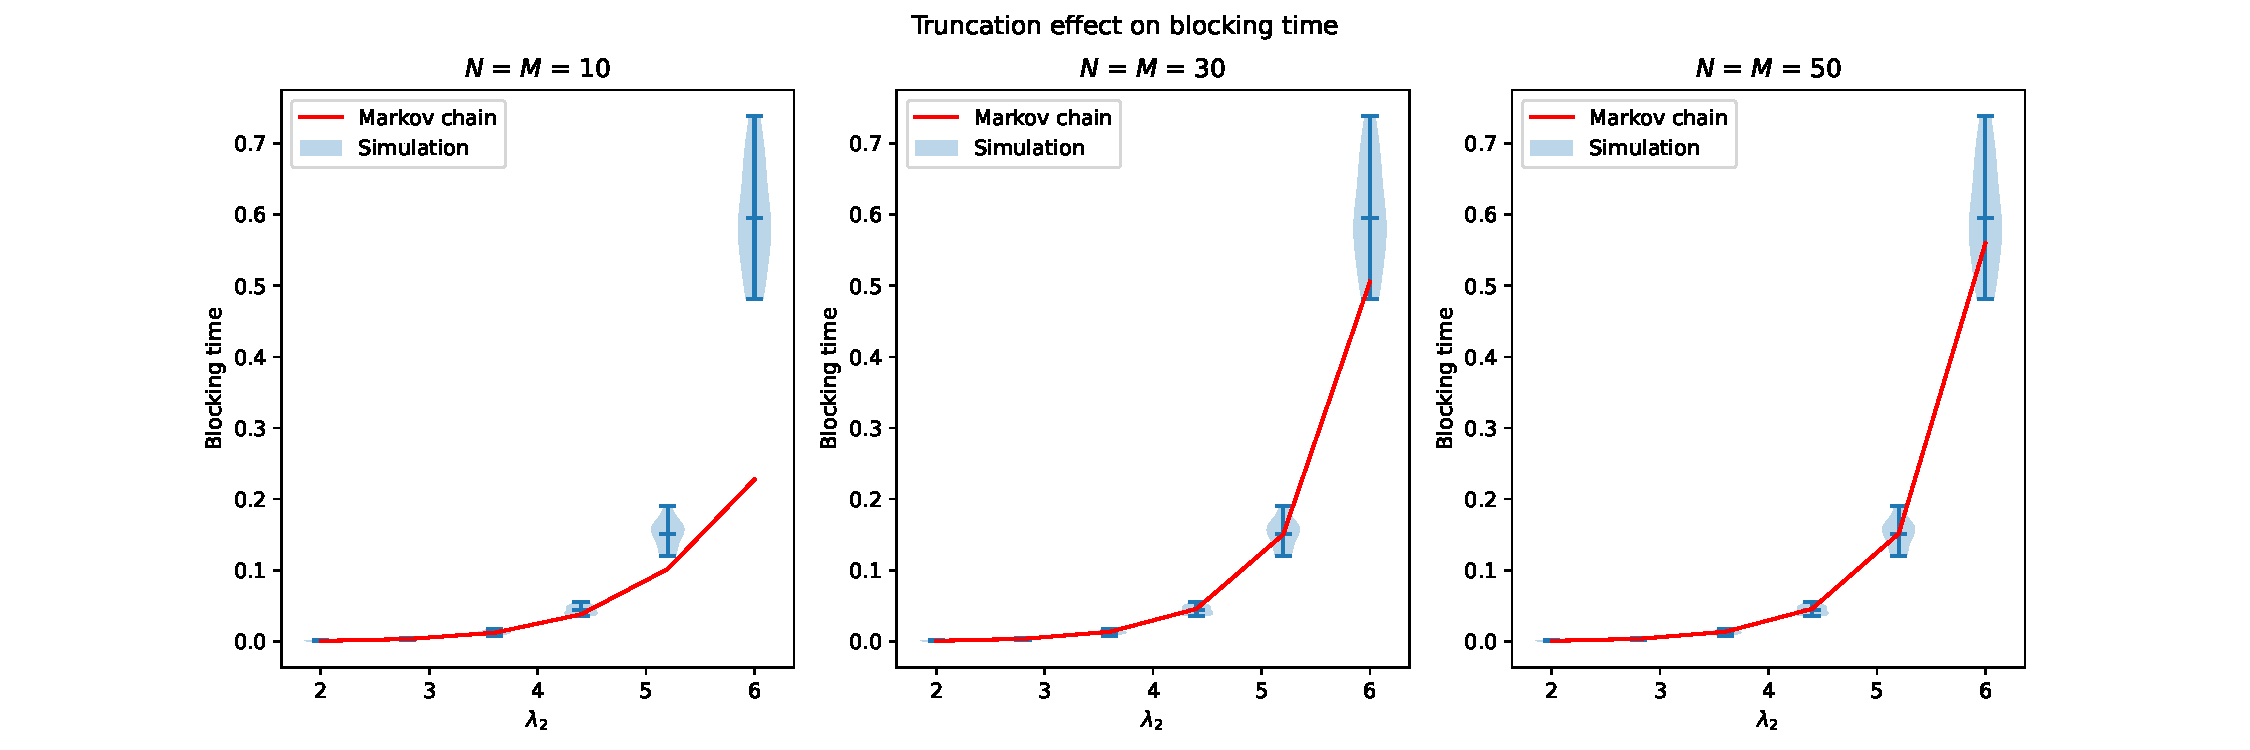
\includegraphics[width=\textwidth]{imgs/truncation_effect/blocking/main.pdf}
    \caption{
        Comparison of mean blocking time between values obtained from the Markov 
        chain formula, values obtained from the truncated simulation and values
        obtained from the untruncated simulation.
    }
    \label{fig:markov_vs_des_blocking_time_comparison}
\end{figure}
